\newpage
\section{Realidad Aumentada}
\setcounter{secnumdepth}{2}

\subsection{Definición}
La realidad aumentada (AR) es una aproximación visual interactiva en tiempo real en la cual objetos virtuales son añadidos al entorno real, normalmente en la parte superior de un video, usando gráficos de computadora o móviles.\cite{B04} \par
\vspace{5mm}
Básicamente la realidad aumentada se refiere a que imágenes virtuales hechas por computadora sean mezcladas con la vista real para crear una visión con elementos agregados. Su principal fundamento es mezclar la realidad con la realidad virtual. Aunque no sólo se trata de mezclar la realidad virtual, también pueden mezclarse elementos como audio, sensaciones, tacto, olores, y gusto los cuales son superpuestos sobre el mundo real para producir un \textbf{entorno de realidad aumentada}.\cite{B05}
Esta tecnología no es nueva, tuvo sus orígenes en la década de los 90s\cite{B04} y su primer aparición a nivel mundial fue en Octubre de 1998 en The FIrst International Workshop on AR (IWAR'98) en San Francisco\cite{B05}.\par 
\vspace{5mm}
La realidad aumentada tiene como objetivo simplificar la vida del usuario al agregar información a su entorno real para su beneficio mediante visión indirecta como la transmisión de video, imagenes, etc. AR mejora la percepción e interacción con el mundo real. Por otro lado la realidad virtual (VR) se sumerge en un entorno puramente virtúal sin interactuar con el mundo real.\cite{B27}\par
\begin{figure}[h!]
	\centering
	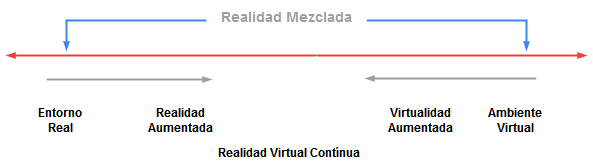
\includegraphics[width=10cm,height=3.5cm]{imagenes/marcoteorico/ar/Mixed_Reallity.png}
	\caption{Milgram’s reality-virtuality continuum.\cite{B27}}
	\label{fig:analogo}
\end{figure}
\subsection{Tecnología de realidad aumentada}
El registro de imágenes de la realidad aumentada utiliza diferentes métodos de visión por computadora, principalmente relacionados con el seguimiento de vídeo. Estos métodos generalmente consisten en dos etapas: reconocimiento y seguimiento/reconstrucción . Primero, se detectan marcadores, imágenes ópticas o puntos de interés en las imágenes de la cámara.\cite{B27} \par
\vspace{5mm}
El reconocimiento puede hacer uso de la detección de características, detección de bordes u otros métodos de procesamiento de imágenes con visión artificial, la mayoría de las técnicas de seguimiento disponibles se pueden separar en dos clases\cite{B27}. \par
\begin{enumerate}[1.]
	\item Basados en caracteristicas
	\item Basados en modelos
\end{enumerate}

\vspace{5mm}
Los métodos basados en características consisten en descubrir la conexión entre las características de imagen en 2D y sus coordenadas del mundo en 3D. \cite{B27} \par
\vspace{5mm}
Los métodos basados en modelos utilizan las características de los objetos rastreados, como pueden ser modelos basados en CAD o las plantillas 2D.En el renderizado 3D es posible encontrar la posición de la cámara, basandonos en la proyección de las coordenadas 3D, de igual forma las coordenadas de imagen observada en 2D  como se aprecia en la imagen 2.5 \cite{B27}.\par
\begin{figure}[h!]
	\centering
	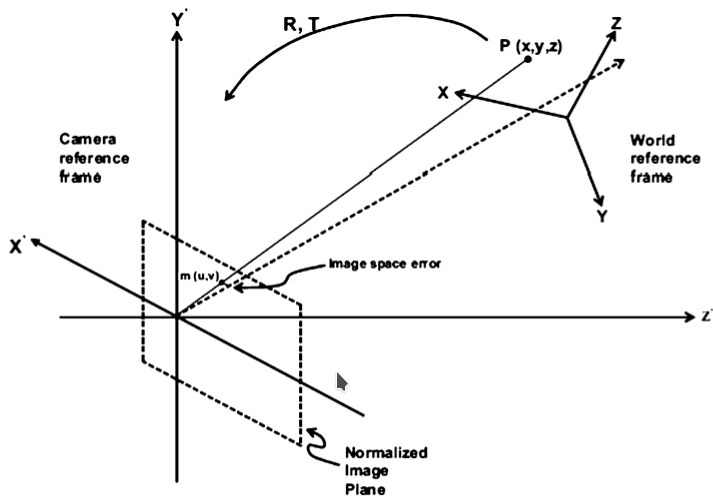
\includegraphics[width=11cm,height=8cm]{imagenes/marcoteorico/ar/tecnologyAR.png}
	\caption{Restricciones de los puntos para el problema de la posición de la cámara respecto al objeto AR.\cite{B27}}
	\label{fig:analogo}
\end{figure}
\subsection{Tipos de Realidad}
Una de las partes más importantes de la realidad aumentada es la capacidad del usuario para ver su entorno. Sin embargo, el dispositivo de realidad aumentada también tiene que "verlo" y eso implica un sistema de visión basado en computadora \cite{B22} .\par
\vspace{5mm}
 Todas las pantallas utilizadas en los sistemas de realidad aumentada portátiles (excluidas por dispositivos móviles de definición tales como teléfonos inteligentes, tabletas y portátiles) son normalmente pantallas transparentes que simulan la vision natura\cite{B22}. \par
\vspace{5mm}
\begin{figure}[h!]
	\centering
	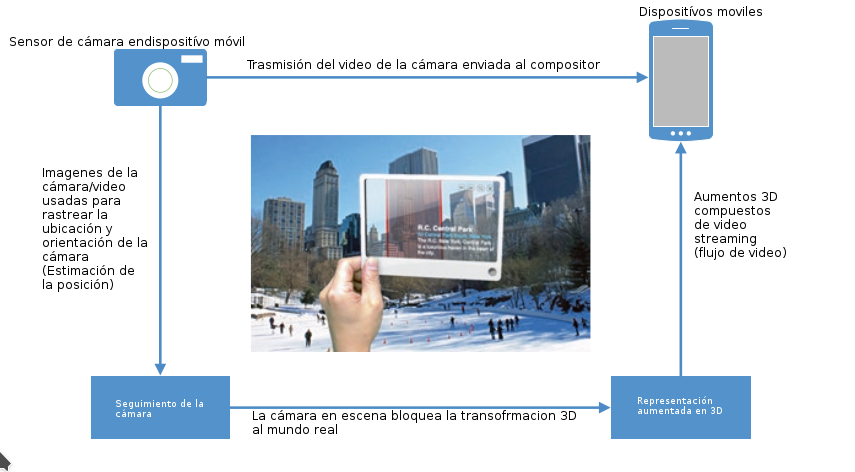
\includegraphics[width=17cm,height=10cm]{imagenes/marcoteorico/ar/visionAR.png}
	\caption{Visión base de la realida aumentada\cite{B22}}
	\label{fig:analogo}
\end{figure}
\subsection{Taxonomía de la realidad aumentada}
La realidad aumentada es un campo sorprendentemente diverso, robusto y complicado. En un nivel superior se encuentran dos categorias principales: Dispositívos protables y dispositívos estacionarios (Moviles y fijos).
Los dispositívos moviles incluyen aquellos como aurículares, cascos y algún día lentes de contacto.Los dispositivos no portátiles (aparatos fijos como televisores, computadoras, reproductores de musica, etc.) y dispositívos móviles (Smartphones, tablet's, notebook's), y pantallas de visualización.El siguiente diagrama describe el campo de la realidad aumentada.\cite{B22} \par
\vspace{5mm}
\begin{figure}[h!]
	\centering
	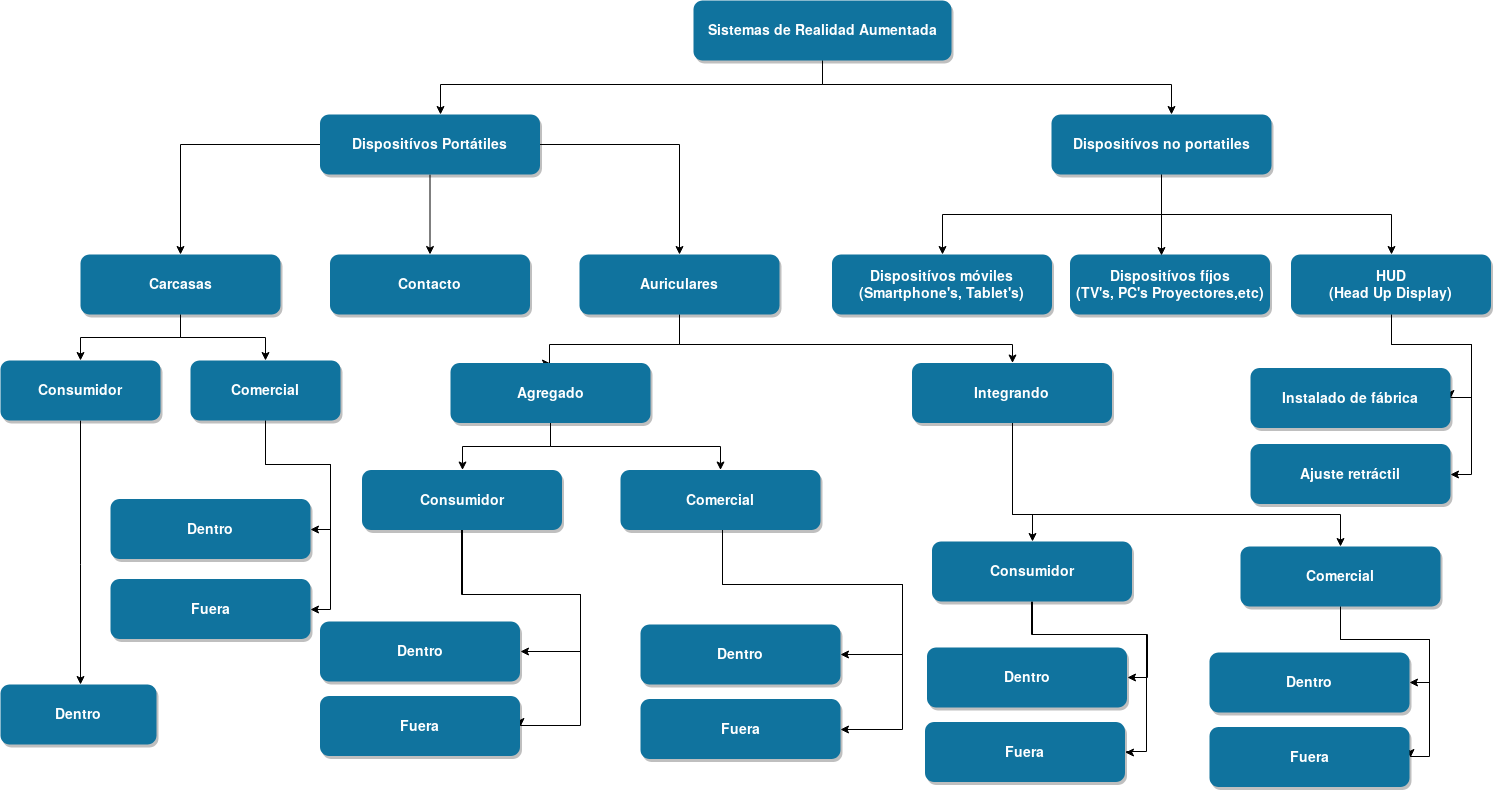
\includegraphics[width=17cm,height=10cm]{imagenes/marcoteorico/ar/taxonomiaAR.png}
	\caption{Taxonomía de la realidad aumentada\cite{B22}}
	\label{fig:analogo}
\end{figure}
La experiencia de la realidad aumentada en dispositivos dedicados o no dedicados como TV's, smarthphones, tablet's y PC's. Dentro de los sistemas de realidad aumentada visuales dedicados, hay siete clases:\cite{B22} \par
\vspace{5mm}
\begin{enumerate}[1.]
	\item Lentes de contacto
	\item Cascos.
	\item Display Head-up (HUD)
	\item Headset(Gáfas inteligentes)
	\begin{enumerate}[a)]
		\item Integrado (interno, externo)
		\item Pantallas y sistemas adicionales para gafas convencionales como sol o de seguridad (interno, externo)
	\end{enumerate}
	\item Proyectores(No HUD)
	\item Dedicados y otros (TV,Salud, alarmas,etc)

\end{enumerate}

El autor Steve Mann nos dice acerca de la realidad aumentada: "Un mediador ideal de la realidad es tal que es capaz de producir un ilusión de transparencia sobre algunos o todos los campos visuales.\cite{B22} \par
\subsection{Impacto de la realidad aumentada}
Desde su aparición en los 90s, la realidad aumentada ha sido una tecnología de punta la cual sólo estaba disponible en algunos laboratorios y de forma remota al público en general. \par
Más allá de ser una útil técnica de visualización, actualmente es usada en muchos sectores como la ingenería, la medicina, la robótica, la milicia, la educación, entretenimiento, etc.\par
La realidad aumentada se ha vuelto una tecnología bastante común, y esto es debido principalmente a la popularidad que tienen los dispositivos inteligentes portátiles (como smartphones y tablets), que ya tienen integradas características como cámaras de video, resolución de alta definición y gran poder computacional que se adecúa al procesamiento de datos relacionados a la realidad aumentada.\par
Hoy, con el software apropiado, la mayoría de los usuarios de dispositivos inteligentes pueden usar ésta tecnología para múltiples propósitos sin tener que comprar otros dispositivos de costos elevados como los HDM (Head Mounte Displays). Adicionalmente con el anuncio de Google Glasses (AR Glasses), se puede inferir que el siguiente nivel de la realidad aumentada será la implementación de la realidad aumentada en pupilentes. Sin embargo puede asumirse que los dispositivos inteligentes seguirán siendo la herramienta dominante para el propósito general de la realidad aumentada en el futúro.\par
Como una poderosa herramienta de visualización, la realidad aumentada es aplicable en muchas áreas del diseño, las propuestas de diseño pueden ser examinadas, naturalmente la realidad aumentada mezcla elementos virtuales previamente renderizados con el entorno real, lo cual la convierte particularmente útil para las áreas del diseño que involucran construcción de entornos tales como el diseño urbano, la arquitectura y el diseño de interiores. Al reemplazar una porción del entorno físico con algún modelo tridimensional, la diferencia entre el estatus actual del entorno y el estatus simulado se vuelve evidente, logrando que sea posible previsualizar un diseño, sin necesidad de llevarlo a cabo.\par
En el campo de la investigación del diseño de interiores, la realidad aumentada ha sido usada para simular objetos dentro de un espacio arquitectónico determinado. Estos objetos a menudo son muebles, accesorios o aparatos. Con el entorno físico capturado por un dispositivo en tiempo real y procesado de forma visual, el renderizado de objetos 3D es superpuesto.\cite{B15}

\subsection{Plataformas de realidad aumentada para dispositivos móvilves}
El impacto y la popularidad de la realidad aumentada han sido tan grandes, que actualmente existen varias plataformas para desarrollar tecnologías que usen realidad aumentada, ya sea para dispositivos móviles como smartphones y tablets, o para dispositivos integradores como los cascos de realidad virtual. Dentro de las plataformas más usadas podemos encontrar:
\begin{itemize}
	\item Wikitude
	\item ARKit
	\item Vuforia
	\item ARToolKit
	\item ARCore
\end{itemize}
\newpage

\subsubsection{Wikitude}
Wikitude es una plataforma de desarrollo de aplicaciones móviles, teniendo como principales dispositivos los smartphones, tabletas y gafas inteligentes. Esta plataforma les otorga a los desarrolladores una combinación única de un mundo físico y virtual. Wikitude se apoya de potentes funciones en combinación con la realidad aumentada (AR), actualmente disponibles para los sistemas Android, iOS, Google Glass, Epson Moverio, Vuzix M-100, Optinvent ORA1, PhoneGap, Titanium y Xamarin. Algunas de estas funciones son:\cite{B09}
\begin{itemize}
	\item \textbf{Escaneo de objetos para su reconocimiento}.- Wikitude proporciona un escaneo de objetos como muebles a través de la cámara de un dispositivo móvil. Las últimas versiones de Wikitude se apoya de \textbf{SLAM Simultaneous Location  and Mapping} que permite un escaneo mas amplio como habitaciones. 
	
	\item \textbf{Seguimiento instantáneo}.- La tecnología Instant Tracking hace posible que las aplicaciones de realidad aumentada trabajen sin necesidad de un marcador, Wikitude utiliza SLAM \textbf{(Simultaneous Localization and Mapping) }esta tecnología mapea las imágenes obtenidas por la cámara de un dispositivo compatible y generar marcas o puntos característicos.
	
	\item \textbf{Reconocimiento 2D}.- El reconocimiento de imágenes por parte de Wikitude proporciona a los desarrolladores el cambiar los ángulos, dimensiones y ubicación de las imágenes virtuales dentro del mundo real obtenida por medio de la cámara del dispositivo en tiempo real.
	
	\item \textbf{Servicios de geolocalización}.- Esta tecnología nos permite combinar la realidad aumentada (AR) combinando datos georreferenciados. Dependiendo del uso que se le de a la aplicación, la ubicación de algo en particular se apoya de la tecnología \textbf(GPS sistema de posicionamiento global). Un ejemplo de este típo de aplicaciones es Pokemon GO. 
	
	\item \textbf{Reconocimiento multi-imagen}.- Esta función de Wikitude permite el reconocimiento de varias imágenes simultáneamente adquiridas por la cámara del dispositivo. Una vez que se reconocen las imágenes, los desarrolladores pueden manipular modelos 3D y combinarlos con el mundo real, este tipo de reconocimiento múltiple de imágenes se puede usar para brindar interactividad a muchas aplicaciones.
	
	\item \textbf{Seguimiento extendido}.- Extended Tracking permite a los desarrolladores ir más allá con la manipulación de imágenes y objetos virtuales, los usuarios mejoran su experiencia de realidad aumentada (AR) moviendo libremente sus dispositivos sin la necesidad de mantener un marcador a la vista de la cámara. Esta función de igual forma se apoya de \textbf{SLAM}. 
	
	\item \textbf{Reconocimiento en la nube}.- El servicio de reconocimiento en la nube de Wikitude permite a los desarrolladores trabajar con miles de imágenes alojadas en la nube y trabaja con un tiempo de respuesta muy rápido.
	
	\item \textbf{Aumentado en 3D}.- Esta tecnología carga y renderiza modelos en 3D sobre la escena proporcionada por la cámara del dispositivo, importando los objetos virtuales desde herramientas de renderizado como \textbf{Autodesk, Maya o Blender 3D}, Wikitude trabaja conjuntamente con Unity3D para integrar animaciones por computadora.\cite{B16}
	
\end{itemize}
\noindent
Wikitude nos ofrece muchas vertientes para el desarrollo de realidad aumentada (AR), actualmente la convierte en una de las mejores tecnologías posicionadas en el mercado. Esta plataforma se puede instalar desde su pagina oficial, existe una versión de prueba y se puede adquirir la licencia desde 2490 euros.\cite{B16} 

Algunos de los dispositivos compatibles con Wikitude se muestran en la siguiente tabla.
\begin{table}[h]
	\begin{tabular}{| p{4.5cm} | p{10.5cm} |}
		\hline \centering
		\textbf{Marca}              & \multicolumn{1}{c|}{\textbf{Modelo}}               \\ \hline \centering
		\multirow{5}{*}{Google}     & Nexus 4+                                \\ \cline{2-2} 														  
		& Nexus 5+                                           	\\ \cline{2-2} 
		& Nexus 6P                                           	\\ \cline{2-2} 
		& Nexus 10+                                          	\\ \cline{2-2} 
		& Google Glass                                       	\\ \hline \centering
		\multirow{1}{*}{Epson}     & Epson Moverio BT-200       \\ \cline{2-2} 
		\hline \centering
		\multirow{3}{*}{Apple}     & iPhone 4+                                \\  \cline{2-2}     														
		& Pad2X			                                    	\\ \cline{2-2} 
		& iPod Touch 5th gen                                 	\\ \hline \centering
		\multirow{1}{*}{Vuzix}         & Vuzix M100          	\\ \cline{2-2}
		\hline \centering
		\multirow{5}{*}{Samsung} 	   & Galaxy S2+           	\\ \cline{2-2} 
		& Galaxy S7, Galaxy S7 edge                          	\\ \cline{2-2} 
		& Galaxy S8, Galaxy S8+                              	\\ \cline{2-2} 
		& Galaxy S9, Galaxy S9+                              	\\ \cline{2-2} 
		& Galaxy Tab S4                                      	\\ \hline \centering
		\multirow{3}{*}{Sony}       & Xperia XZ Premium                                  \\ \cline{2-2} 
		& Xperia XZ1, Xperia XZ1 Compact                     \\ \cline{2-2} 
		& Xperia XZ2, Xperia XZ2 Compact, Xperia XZ2 Premium \\ \hline
	\end{tabular}
	\captionsetup{justification=centering}
	\caption{Listado de dispositivos compatibles con Wikitude}
\end{table}

\subsubsection{ARKit} ARKit 2 es la plataforma nativa de los sistemas \textbf{iOS} para el desarrollo de realidad aumentada (AR). Esta API nos proporciona una experiencia única en los objetos 3D incluyendo reflejos de entorno del mundo real en objetos virtuales brillantes, incluso la capacidad de interactuar con varios usuarios en tiempo real. Actualmente ARKit se encuentra en su versión 2 y con soporte exclusivo para los sistemas \textbf{iOS 12} y posteriores.\cite{B20}
\begin{itemize}
	\item \textbf{Experiencias de AR compartidas}.-Las aplicaciones de AR ya no están limitadas a una sola persona o dispositivo, actualmente ARKit proporciona experiencias multiusuario como juegos donde las experiencias de realidad aumentada se extienden hasta poder ser participe como un espectador.\cite{B20}
	\item \textbf{Experiencias de AR persistentes}.-
	ARKit proporcionar experiencias de AR persistentes  mediante una sesión  y sea capaz de reanudarla más adelante, por ejemplo los usuarios pueden iniciar un rompecabezas AR en una mesa y volver a él en el mismo estado que se dejo.\cite{B20}
	\item \textbf{Detección y Seguimiento de Objetos}.- Desde su versión 1.5  ARKit agregó soporte para la detección de imágenes 2D, lo que le permite desencadenar una experiencia de realidad aumentada basada en imágenes 2D y aplicarlas en  carteles, obras de art, etc. ARKit proporciona un seguimiento dinámico total de imágenes en 2D, de modo que objetos virtuales móviles se podrán observar en nuestro mundo real. ARKit  también agrega la capacidad de detectar objetos 3D dentro de un catalogo, como esculturas, juguetes o muebles.\cite{B20}
	\item \textbf{Detección y Seguimiento de Objetos}.- Desde su versión 1.5  ARKit agregó soporte para la detección de imágenes 2D, lo que le permite desencadenar una experiencia de realidad aumentada basada en imágenes 2D y aplicarlas en  carteles, obras de art, etc.ARKit 2 proporciona un seguimiento dinámico total de imágenes en 2D, de modo que objetos virtuales móviles se podrán observar en nuestro mundo real. ARKit también agrega la capacidad de detectar objetos 3D dentro de un catalogo, como esculturas, juguetes o muebles.\cite{B20}
	\item \textbf{Quick Look en objetos 3D y AR}.- Las experiencias de objetos 3D y realidad aumentada (AR) de forma nativa para \textbf{iOS} ofrece una optimización de almacenamiento, usted puede compartir estas experiencias en mensajes, correos, noticias, etc. Con la tecnologia \textbf{Quick Look} los usuarios ven experiencias detalladas e increíbles, incluyendo reflejos del entorno del mundo real en objetos virtuales.\cite{B20}
\end{itemize}
\begin{table}[h]
	\begin{tabular}{| p{4.5cm} | p{10.5cm} |}
		\hline \centering
		\textbf{Marca}              & \multicolumn{1}{c|}{\textbf{Modelo}}               \\ \hline \centering
		\multirow{16}{*}{Apple}       & iPhone 6     \\ \cline{2-2}  
		& iPhone 6 Plus                                 \\ \cline{2-2}
		& iPhone 6S                                     \\ \cline{2-2}
		& iPhone 6S Plus                                \\ \cline{2-2}
		& iPhone 7                                      \\ \cline{2-2}
		& iPhone 7 Plus                                 \\ \cline{2-2}
		& iPhone 8                                      \\ \cline{2-2}
		& iPhone 8 Plus                                 \\ \cline{2-2}
		& iPhone X                                      \\ \cline{2-2}
		& iPad Pro 12.9                                 \\ \cline{2-2}
		& iPad Pro 12.9 (2nd Gen)                       \\ \cline{2-2}
		& iPad Pro 10.5                                 \\ \cline{2-2}
		& iPad Pro 9.7                                  \\ \cline{2-2}
		& iPad (3rd Gen)	                              \\ \cline{2-2}
		& iPad (4th Gen)	                              \\ \cline{2-2}
		& iPad Air                                      \\ \cline{2-2}
		\hline 
	\end{tabular}
	\captionsetup{justification=centering}
	\caption{Listado de dispositivos compatibles con ARKit 2}
\end{table}
\noindent
\subsubsection{Vuforia}
Vuforia es una API que integra un motor Unity3D para su desarrollo con realidad aumentada (AR), sus aplicaciones están escritas en C sin embargo es multiplataforma.\par
	\begin{itemize}
	
	\item \textbf{Objetivos}.- Un Target es un patrón de características naturales predefinidas por el desarrollador o usuario. El buscador de  Vuforia asocia una determinada a una imagen u objeto,a  su vez el software necesita saber qué patrones buscar. Para este propósito, los desarrolladores pueden usar el administrador de objetivos de Vuforia, de igual forma ofrece a los desarrolladores un servicio web para crear objetivos a partir de imágenes 2D, cuboides, cilindros y objetos tridimensionales.
	
	\item \textbf{Rastreo Extendido}.- El rastreo es una función que permite a Vuforia encontrar objetivos utilizando las características especificas y se  puede construir un mapa de características que rodean al objetivo a escanear y mantener la detección aunque no esté dentro de la vista de la cámara, 
	
	\item \textbf{Reconocimiento de imágenes}.- Vuforia contiene un administrador de objetivos, se puede definir un objetivo de imagen utilizando cualquier patrón, la composición y la cantidad de características son los factores decisivos en la facilidad con que Vuforia puede detectar un objetivo de imagen.
	
	\item \textbf{Reconocimiento de Objetos}.- Si bien el reconocimiento de objetos de Vuforia utiliza el seguimiento de funciones naturales en su núcleo, el proceso de creación de objetos objetivos es bastante diferente en comparación con la creación de objetos de imágenes virtuales. Una imagen contiene características en 2D mediante el análisis de los pixeles del archivo de imagen proporcionado al administrador de destino. Sin embargo, un objeto 3D tiene un tercer eje a considerar. Los objetivos de objeto permiten a los usuarios ver objetos aumentados desde varios ángulos mientras el objeto mantiene su aumento. Antes de aumentar objetos 3D, Vuforia ha desarrollado una aplicación de escaneo que es capaz de obtener los objetos relativamente pequeños usando un cierto "plano de escaneo" sobre el cual se coloca el objeto a escanear, el objeto a ser escaneado sobre el objetivo de la imagen, el escáner de Vuforia puede determinar la coordenada XYZ, representada por un punto verde.\par
	Vuforia se apoya de un patron o marca como un objetivo detectable por la aplicación. Vuforia trabaja con la posición y orientación, como marco de referencia utiliza un sistema de coordenadas 2D. Algunas de las funciones mas importantes para entender el alcance de esta librería. \cite{B12}
	Algunos de los dispositivos compatibles con Vuforia se muestran a continuación.
\end{itemize}
\begin{table}[h]
	\begin{tabular}{| p{4.5cm} | p{10.5cm} |}
		\hline \centering
		\textbf{Marca}              & \multicolumn{1}{c|}{\textbf{Modelo}}               \\ \hline \centering
		\multirow{1}{*}{Asus}         & Asus ZenFone AR         	\\ \cline{2-2}
		\hline \centering
		\multirow{3}{*}{Xiaomi} & Xiaomi Redmi 3S    \\ \cline{2-2}
		& Xiaomi Redmi Note 3  \\ \cline{2-2}
		& Xiaomi Redmi Note 3 Snapdragon     \\ \hline \centering
		\multirow{7}{*}{Huawei} & Huawei Mate 10   \\ \cline{2-2}
		& Huawei Mate 10 Pro   \\ \cline{2-2}
		& Huawei P10   \\ \cline{2-2}
		& Huawei P10 Lite   \\ \cline{2-2}
		& Huawei P20 Lite   \\ \cline{2-2}
		& Huawei P20   \\ \cline{2-2}
		& Huawei P20 Pro \\ \hline 
	\end{tabular}
\captionsetup{justification=centering}
\caption{Listado de dispositivos compatibles con Vuforia}
\end{table}

\begin{table}[]
	\begin{tabular}{| p{4.5cm} | p{10.5cm} |}
		\hline \centering
		\textbf{Marca}              & \multicolumn{1}{c|}{\textbf{Modelo}}               \\ \hline \centering
		\multirow{7}{*}{Huawei} & Huawei Mate 10   \\ \cline{2-2}
		& Huawei Mate 10 Pro   \\ \cline{2-2}
		& Huawei P10   \\ \cline{2-2}
		& Huawei P10 Lite   \\ \cline{2-2}
		& Huawei P20 Lite   \\ \cline{2-2}
		& Huawei P20   \\ \cline{2-2}
		& Huawei P20 Pro  \\ \hline   \centering
		\multirow{1}{*}{Motorola}     &  Motorola Moto G4  \\ \cline{2-2}
		\hline \centering
		\multirow{4}{*}{LG}  & LG V30      \\ \cline{2-2}
		& LG G6   \\ \cline{2-2}
		& LG G7  \\ \cline{2-2}
		& LG G8                        \\ \hline   \centering
		\multirow{2}{*}{OPPO}   & OPPO R11      \\ \cline{2-2}
		& OPPO R11t         \\   \hline \centering
		\multirow{2}{*}{Sony}   & Xperia Z5      \\ \cline{2-2}
		& Xperia XZ      \\ \hline \centering
		\multirow{23}{*}{Apple}     & iPad Air 2     \\ \cline{2-2}
		& iPad Mini   \\ \cline{2-2}
		& iPad Mini 2   \\ \cline{2-2}
		& iPad Mini 3   \\ \cline{2-2}
		& iPad Mini 4   \\ \cline{2-2}
		& iPhone 5   \\ \cline{2-2}
		& iPhone 5c   \\ \cline{2-2}
		& iPhone 5s   \\ \cline{2-2}
		& iPhone SE   \\ \cline{2-2}
		& iPhone 6   \\ \cline{2-2}
		& iPhone 6 Plus   \\ \cline{2-2}
		& iPhone 6S   \\ \cline{2-2}
		& iPhone 6S Plus   \\ \cline{2-2}
		& iPhone 7   \\ \cline{2-2}
		& iPhone 7 Plus   \\ \cline{2-2}
		& iPhone 8    \\ \cline{2-2}
		& iPhone 8 Plus   \\ \cline{2-2}
		& iPhone X   \\ \cline{2-2}
		& iPad Pro 12.9   \\ \cline{2-2}
		& iPad Pro 12.9 (2nd Gen)   \\ \cline{2-2}
		& iPad Pro 10.5   \\ \cline{2-2}
		& iPad Pro 9.7   \\ \cline{2-2}
		& iPad (3rd Gen)   \\ \cline{2-2}
		& iPad (4th Gen)   \\ \cline{2-2}
		& iPad (5th Gen)  \\  \cline{2-2}
		& iPad Air   \\ \cline{2-2}
		& iPod Touch (5th Gen)   \\ \cline{2-2}
		& iPod Touch (6th Gen)   \\ \hline 
	\end{tabular}
	\captionsetup{justification=centering}
	\caption{Listado de dispositivos compatibles con Vuforia}
\end{table}
\newpage
\begin{table}[]
	\begin{tabular}{| p{4.5cm} | p{10.5cm} |}
		\hline \centering
		\textbf{Marca}              & \multicolumn{1}{c|}{\textbf{Modelo}}               \\ \hline \centering
\multirow{5}{*}{Samsumg}     & Samsung Galaxy J5 Pro                       \\ \cline{2-2} 														  
& Samsung Galaxy S6   \\ \cline{2-2}
& Samsung Galaxy S6 Edge   \\ \cline{2-2}
& Samsung Galaxy S6 Edge+   \\ \cline{2-2}
& Samsung Galaxy A7   \\ \cline{2-2}
& Samsung Galaxy J7 Pro   \\ \cline{2-2}
& Samsung Galaxy S7   \\ \cline{2-2}
& Samsung Galaxy S7 Edge - Exynos   \\ \cline{2-2}
& Samsung Galaxy S7 Edge - Snapdragon   \\ \cline{2-2}
& Samsung Galaxy A8+   \\ \cline{2-2}
& Samsung Galaxy S8   \\ \cline{2-2}
& Samsung Galaxy S8+   \\ \cline{2-2}
& Samsung Galaxy S9   \\ \cline{2-2}
& Samsung Galaxy S9+   \\ \cline{2-2}
& Samsung Galaxy Note 5 – Exynos   \\ \cline{2-2}
& Samsung Galaxy Note 8   \\ \cline{2-2}
& Samsung Galaxy Note 9    \\ \cline{2-2}
& Galaxy Tab S3 9.7  \\ \hline   \centering
\multirow{5}{*}{Google}    & Google Pixel              \\ \cline{2-2}
& Google Pixel XL   \\ \cline{2-2}
& Google Pixel 2   \\ \cline{2-2}
& Google Pixel 2 XL   \\ \cline{2-2}
& Google Nexus 6P    \\ \hline 
\end{tabular}
\captionsetup{justification=centering}
\caption{Listado de dispositivos compatibles con Vuforia}
\end{table}

\newpage
\noindent


\subsubsection{ARCore}
ARCore es la plataforma de Google para construir experiencias de realidad aumentada. A través de diferentes APIs, ARCore le da la habilidad a un dispositivo móvil para percibir su entorno, entender el mundo e interactuar con la información. Algunas de nuestras APIs están disponibles a través de Android y iOS para crear experiencias de realidad aumentada compartidas \cite{B14}.\par
ARCore tiene nueve pilares básicos que permiten integrar contenido virtual en el entorno real, por medio de la cámara de un dispositivo móvil:

\begin{itemize}
	\item \textbf{Rastreo de movimiento}.- Cuando el celular se mueve a través del mundo real, ARCore usa un proceso llamado \textbf{Odometría concurrente y mapeo} o simplemente \textbf{COM}, para entender en qué posición se encuentra con respecto al entorno. ARCore detecta visualmente distintas características en las imágenes capturadas por la cámara para definir puntos llamados \textbf{puntos característicos}, a partir de los cuales virtualmente genera una maya de puntos, y los usa para computar el cambio físico de su posición. Esto se combina con mediciones realizadas por el teléfono para determinar la posición y la orientación de la cámara relativa al mundo en tiempo real.
	
	\item \textbf{Entendimiento ambiental}.- ARCore trata de identificar una maya de puntos coincidentes dentro de una misma superficies, como una mesa, el suelo o un muro, y hace que cada una de estas superficies detectadas esté disponible como un \textbf{plano}. ARCore también es capaz de detectar los límites de cada plano y convertir esto en información útil para las aplicaciones, de tal forma que sea posible posicionar objetos virtualmente sobre cada uno de estos planos. Debido a que ARCore usa puntos característicos para detectar planos, superficies sin texturas como paredes blancas pueden no ser detectadas apropiadamente.
	
	\item \textbf{Estimación de luz}.- ARCore puede detectas información sobre la iluminación del entorno y proveer a la cámara de dispositivo móvil de una corrección de color y gamma, para lograr una imagen óptima. Esta información permite variar la iluminación de una habitación y ver cómo la iluminación también varía en los elementos virtuales, aumentando la sensación de realismo.
	
	\item \textbf{Interacción con el usuario}.- Una vez que se ha definido la maya de puntos, ARCore permite que el usuario interactue con el entorno visualizado en la cámara del dispositivo. El usuario puede hacer tap, o realizar gestos con los dedos sobre la pantalla del móvil, y ARCore tiene la capacidad de interpretar y transportar éstas acciones al entorno virtual, por ejemplo, el usuario puede agregar un objeto en alguna superficie al tocar la pantalla del dispositivo con el dedo, tras esto se hace una cálculo de las coordenadas relativas X, Y del plano donde se va a agregar el objeto, y finalmente el objeto es mostrado a través de la cámara.
	
	\item \textbf{Puntos de orientación}.- Los puntos de orientación permiten colocar objetos virtuales en superficies inclinadas. Cuando se está detectando la maya de puntos y se detectan superficies cercanas con diferente ángulo, ARCore se encarga de calcular el ángulo de inclinación de tal superficie.
	
	\item \textbf{Anclas y rastreables}.- La posición y orientación puede cambiar conforme ARCore mejora su entendimiendo del entorno. Cuando se quiere posicionar un objeto virtual, se requiere definir una ancla para asegurar que su posición sea rastreada en tiempo real. Los planos y puntos son un tipo de objeto especial denominado \textbf{rastreable}. Como su nombre sugiere, son objetos que ARCore estará rastreando a lo largo del tiempo. Es posible anclar objetos a rastreables, de tal forma que estos objetos virtuales van a conservar su posición relativa en el mundo, no importando si la cámara se mueve e inclusive si estos salen del foco de visualización.
	
	\item \textbf{Imágenes aumentadas}.- Las imágenes aumentadas permiten desarrollar aplicaciones de realidad aumentada que puedan responder a imágenes en 2D específicas como paquetes o posters de películas. Los usuarios pueden tener experiencias de realidad aumentada cuando ellos enfocan la cámara del celular a uno de estos elementos, por ejemplo, al enfocar la cámara el póster de una película se puede hacer que un personaje aparezca dentro del entorno virtual, y desaparezca cuando la cámara deje de enfocar a la imagen.
	
	\item \textbf{Compartir}.- \textbf{Cloud Anchors API}) permite crear experiencias de realidad aumentada colaborativas con otras personas. Con ésta API, un dispositivo puede enviar un ancla y puntos característicos a a la nube. Éstas anclas pueden ser compartidas con otros usuarios ya sea de Android o iOS. Esto habilita a las apps para renderizar los mismos objetos 3D asociados a tales anclas, permitiendo a los usuarios tener la misma experiencia de realidad aumentada de forma simultánea
	
\end{itemize}

\noindent
Dado que ARCore es una tecnología nueva (su primer publicación oficial fue en febrero de 2018 y su primer versión estable fue en agosto de 2018) la lista de dispositivos compatibles con ella no es tan amplia. En la \textit{Tabla 2} podemos observar una lista con los dispositivos que actualmente soportan ARCore.
\begin{table}[h]
	\begin{tabular}{| p{4.5cm} | p{10.5cm} |}
		\hline \centering
		\textbf{Marca}              & \multicolumn{1}{c|}{\textbf{Modelo}}               \\ \hline \centering
		\multirow{2}{*}{ASUS}       & Zenfone AR                                         \\ \cline{2-2} 
		& Zenfone ARES                                       \\ \hline  \centering
		\multirow{4}{*}{Google}     & Nexus 5X                                           \\ \cline{2-2} 
		& Nexus 6P                                           \\ \cline{2-2} 
		& Pixel, Pixel XL                                    \\ \cline{2-2} 
		& PIxel 2, Pixel 2 XL                                \\ \hline \centering
		\multirow{4}{*}{LG}         & G6                                                 \\ \cline{2-2} 
		& G7 ThiQ                                            \\ \cline{2-2} 
		& V30, V30+, V30+ JOJO                               \\ \cline{2-2} 
		& V35 ThinQ                                          \\ \hline  \centering
		\multirow{5}{*}{HDM Global} & Nokia 6                                            \\ \cline{2-2} 
		& Nokia 6.1 Plus                                     \\ \cline{2-2} 
		& Nokia 7 Plus                                       \\ \cline{2-2} 
		& Nokia 8                                            \\ \cline{2-2} 
		& Nokia 8 Sirocco  \\ \hline
	\end{tabular}
\captionsetup{justification=centering}
\caption{Listado de dispositivos compatibles con ARCore}
\end{table}
\newpage
\begin{table}[]
	\begin{tabular}{| p{4.5cm} | p{10.5cm} |}
		\hline \centering
		\textbf{Marca}              & \multicolumn{1}{c|}{\textbf{Modelo}}               \\ \hline  \centering
		\multirow{4}{*}{Huawei}     & Honor 10                                           \\ \cline{2-2} 
		& nova 3, nova 3i                                    \\ \cline{2-2} 
		& P20, P20 Pro                                       \\ \cline{2-2} 
		& Porsche Design Mate RS                             \\ \hline  \centering
		\multirow{7}{*}{Motorola}   & Moto GS5 Plus                                      \\ \cline{2-2} 
		& Moto G6                                            \\ \cline{2-2} 
		& Moto G6 Plus                                       \\ \cline{2-2} 
		& Moto X4                                            \\ \cline{2-2} 
		& Moto Z2 Force                                      \\ \cline{2-2} 
		& Moto Z3                                            \\ \cline{2-2} 
		& Moto Z3 Play                                       \\ \hline  \centering
		\multirow{4}{*}{OnePlus}    & OnePlus 3T                                         \\ \cline{2-2} 
		& OnePlus 5                                          \\ \cline{2-2} 
		& OnePlus 5T                                         \\ \cline{2-2} 
		& OnePlus 6                                          \\ \hline  \centering
		\multirow{10}{*}{Samsung}   & Galaxy A5                                          \\ \cline{2-2} 
		& Galaxy A6                                          \\ \cline{2-2} 
		& Galaxy A7                                          \\ \cline{2-2} 
		& Galaxy A8, Galaxy A8+                              \\ \cline{2-2} 
		& Galaxy Note8                                       \\ \cline{2-2} 
		& Galaxy Note9                                       \\ \cline{2-2} 
		& Galaxy S7, Galaxy S7 edge                          \\ \cline{2-2} 
		& Galaxy S8, Galaxy S8+                              \\ \cline{2-2} 
		& Galaxy S9, Galaxy S9+                              \\ \cline{2-2} 
		& Galaxy Tab S4                                      \\ \hline  \centering
		\multirow{3}{*}{Sony}       & Xperia XZ Premium                                  \\ \cline{2-2} 
		& Xperia XZ1, Xperia XZ1 Compact                     \\ \cline{2-2} 
		& Xperia XZ2, Xperia XZ2 Compact, Xperia XZ2 Premium \\ \hline
	\end{tabular}

\captionsetup{justification=centering}
\caption{Listado de dispositivos compatibles con ARCore}
\end{table}
